\chapter{Vorbereitungs-Testphase der Anwendungen}\label{sec:pre-study}

Dieser Abschnitt beschreibt eine vorbereitende Testphase, die den im folgenden Kapitel  \ref{sec:study} dargestellten Versuchsdurchführung vorgelagert ist. Ziel dieser Phase war es, erste
gebrauchstauglichkeitsbezogene Probleme der entwickelten Anwendung zu identifizieren. Auf diese Weise sollen potenzielle Schwächen frühzeitig erkannt werden, um vor Beginn der eigentlichen Testreihen entsprechende Anpassungen vorzunehmen oder relevante Aspekte gezielt in die Versuchsdurchführung zu integrieren.

\section{Methodik}
In diesem Kapitel wird die methodische Herangehensweise der vorbereitenden Testphase dargestellt, mit dem Fokus auf die Identifikation erster gebrauchstauglichkeits-bezogener Schwächen sowohl der Anwendungen, des infrastrukturellen Aufbaus und der Rätsel. Ziel war es, die technische Infrastruktur bereitzustellen und durch erste Testspielsitzungen einen Eindruck von der Schwierigkeit der Rätsel sowie der Bedienbarkeit der Anwendung zu gewinnen. Hierzu wurde ein qualitatives Erhebungsverfahren angewandt.

\subsection{Forschungsdesign}

Um erste gebrauchstauglichkeitsbezogene Schwächen der Anwendung identifizieren zu können, wurde das praxisorientierte Thinking-Aloud-Verfahren eingesetzt. Der Fokus lag dabei insbesondere auf der Evaluation der implementierten Steuerungselemente der Player- und Watcher-Anwendungen, sowie der Rätsel.

\subsection{Erhebnungsinstrumente}

Zur Erfassung der im Rahmen der Thinking-Aloud-Methode geäußerten Gedanken und Hinweise der Probanden, wurde ein Beobachtungsprotokoll als Erhebungsinstrument eingesetzt. Die verbalen Äußerungen wurden stichpunktartig dokumentiert, wobei der Fokus auf spontanen Kommentaren zur Steuerung, zu den Rätseln sowie zu aufgetretenen  Schwierigkeiten lag. Auf eine audiovisuelle Aufzeichnung wurde bewusst verzichtet, um die Testsituation möglichst natürlich zu gestalten. Die protokollierten Aussagen wurden anschließend einer qualitativen Inhaltsanalyse unterzogen.

\subsection{Stichporengröße}\label{sec:pre-study-sample}

Bei der Festlegung der Stichprobengröße musste der Aspekt des \say{Verbrauchens von Probanden} berücksichtigt werden, da die ausgewählten Teilnehmer nicht an der späteren Hauptuntersuchung teilnehmen durften. Aufgrund ihrer Vorerfahrung mit dem Anwendungsszenario bestünde die Gefahr einer Voreingenommenheit, wodurch die Ergebnisse der späteren Wirkungsanalyse verfälscht werden könnten. Aus diesem Grund wurde eine möglichst kleine Stichprobe gewählt, die dennoch in der Lage war, alles relevanten Aspekte der Gebrauchstauglichkeit abzudecken. Entsprechend der Empfehlung \citet[S. 3088]{turner_determining_2006} wurden sieben Probanden rekrutiert, die die erste Version des Prototyps testeten.

\subsection{Durchführung der Studie}

Für die initialen Testdurchläufe wurden gezielt Teilnehmer aus dem näheren Umfeld rekrutiert. Diese verfügten teilweise bereits über Vorkenntnisse hinsichtlich des Themas des Prototyps bzw. der übergeordneten Studie oder waren in der vorangegangenen Projektphase involviert.

Die Tests wurden in Dyaden durchgeführt, wobei die Teilnehmer nacheinander ihre jeweilige Spielerrolle übernahmen. Nach einer kurzen Begrüßung erhielten sie eine Einführung in die Hintergrundgeschichte des Prototyps sowie eine Erläuterung der grundlegenden Steuerung. Anschließend nahmen die Teilnehmer an den jeweiligen Geräten Platz und begannen mit dem Testdurchlauf.

Während des Spielens wurden sie gebeten, ihre Gedanken laut auszusprechen. Die geäußerten Kommentare wurden vom Versuchsleiter, der Reihe nach wie ausgesprochen, dokumentiert.

Nach Abschluss des Durchlaufs wurden die Teilnehmer verabschiedet und die nächste Dyade wurde in den Testraum gebeten. Ein Testdurchlauf pro Dyade nahm 45 Minuten in Anspruch.

\subsection{Rahmenbedingungen}\label{sec:pre-study-rahmen}

Die Durchführung der Prototyp-Test erfolgte im I-Bau der ehemaligen Fakultät\ac{DM}, konkret im Masterpool. Die Tests wurden nach regulären Lehrveranstaltungen und Besprechungen angesetzt, sodass eine ruhige und ungestörte Testumgebung gewährleistet war.

Für die Testdurchführung war umfangreiche Hardware erforderlich, welche über die \ac{DM}-IT sowie das \ac{IIIUS} bereitgestellt wurde. Über die IT konnten ein PC, Monitor, Tastatur und Maus ausgeliehen werden, über die der Player die Anwendung steuert. Das \ac{IIIUS} stellte ein Google Pixel 2 XL, ein Stativ sowie eine Sony-Kamera zur Verfügung, über die der Watcher auf seine Anwendung zugreifen konnte.

Ein TP-Link Router wurde von einem Dozenten der Fakultät \ac{DM} zur Verfügung gestellt, um ein lokales Netzwerk aufzubauen. Dies war notwendig, da sich de Anwendungen beider Rollen im selben Netzwerk befinden mussten, um über den WebSocket-Server kommunizieren zu können. Das hochschulinterne Netzwerk erlaubte keine direkte Verbindung zwischen Endgeräten. Die serverseitige Infrastruktur, bestehend aus einem Docker-Container mit MongoDB sowie dem Node.js-basierten WebSocket-Server, lief auf einem privaten Laptop.

Zur Steuerung der Spielfigur des Players wurde zusätzlich ein 15-Zoll Touchmonitor von Wimaxit verwendet. Die Teilnehmer der Dyade wurden so positioniert, dass sie sich gegenüber saßen und keinen Einblick in die Anwendung der jeweils anderen Person erhalten konnten.

\section{Ergebnisse}\label{sec:pre-study-method-results}

In diesem Abschnitt werden die bei der ersten Prototypversion identifizierten Probleme dargestellt.

Die freiwilligen Probanden waren Studierende der \ac{HFU} (5 weibliche, 2 männliche, im Alter zwischen 22 und 29 Jahren).

Für die Auswertung der Stichpunkte wurde das Verfahren der thematischen Analyse nach \cite{braun_using_2006} herangezogen. Die Analyse erfolgte in sechs Schritten: (1) Vertrautmachen mit den Daten, (2) Generierung erster Codes, (3) Suche nach übergeordneten Themen, (4) Überprüfung der Themen, (5) Definition und Benennung der Themen, sowie (6) abschließende Ergebnisdarstellung.

\begin{figure}[ht]
\centering
\includegraphics[width=1\linewidth]{content/pictures/Prestudy-Qualitative-Auswertung-Schritt-1.png}
\caption{Ergebnis der groben Kategorisierung nach \citealp{braun_using_2006} der Notizen aus Anhang \ref{sec:append_evaluation_pre_study_notes}: \nameref{sec:append_evaluation_pre_study_notes} (Quelle: eigene Darstellung)}
\label{fig:pre-study-qualitative-findings}
\end{figure}

Abbildung \ref{fig:pre-study-qualitative-findings} fasst die von den Teilnehmern geäußerten Aspekte zusammen. Ergänzt wurden diese um weitere Beobachtungen, die während der Tests auffielen, jedoch nicht explizit angesprochen wurden. Die gesammelten Aspekte lassen sich vier Hauptkategorien zuordnen: Environmental / Rätsel, Steuerung, UI und Benennungen. In allen Bereichen wurden Verbesserungsvorschläge formuliert, die vor der Durchführung der groß angelegten Nutzerstudie umgesetzt werden sollten.

Besondere Relevanz kommt den Aspekten der Steuerung zu, insbesondere der Dreh- und Zoom-Funktion innerhalb der Watcher-Anwendung. Darüber hinaus benötigen das Rätsel im Sicherheitsraum sowie das Uhrenrätsel klarere Hinweise und Anpassungen in der Lösungsstruktur.

Weitere Punkte betreffen kleinere bis mittlere kosmetische Optimierungen zur Verbesser der Nutzererfahrung. So waren einige Tooltips nicht korrekt oberhalb der Raumwände positioniert. Auch gestalteten sich die Starträume zu ähnlich, was ihrer Unterscheidbarkeit erschwerte. Ferner bedürfen verschiedene Benennungen im Startbildschirm einer Überarbeitung, um Missverständnisse zu vermeiden.

Die Benutzeroberfläche der Nachrichtenanzeige weist zudem Verbesserungsbedarf in der Kontrastgestaltung von Hintergrund und Schrift auf. Für die Watcher-Anwendung wurde darüber hinaus ein Übersichtsmenü angeregt, in dem empfangene Nachrichten nachgelesen werden können.

In der Player-Anwendung fiel negativ auf, dass bei der Navigation des Avatars eine Fehlermeldung erscheint, wenn auf unereichbare Bereiche geklickt wird. Das Navigieren sollte benutzerfreundlicher gestaltet werden.

\begin{figure}[ht]
\centering
\includegraphics[width=1\linewidth]{content/pictures/Prestudy-Qualitative-Auswertung-Schritt-2.png}
\caption{Ergebnis der feinen Kategorisierung nach \cite{braun_using_2006} (Quelle: eigene Darstellung)}
\label{fig:pre-study-qualitative-findings_2}
\end{figure}

Eine detaillierte Kategorisierung der identifizierten Aspekte ist in Abbildung \ref{fig:pre-study-qualitative-findings_2} dargestellt.

\section{Handlungsempfehlungen}

Aus den gesammelten Ergebnissen lassen sich konkreten Handlungsempfehlungen ableiten, die vor der Durchführung der groß angelegten Nutzerstudie umgesetzt werden sollten.

Im Kontext der Verbesserung der Gebrauchstauglichkeit wurden diese Empfehlungen nach einem Severity Ranking priorisiert, wie in Abbildung \ref{fig:handlungsempfehlungen-vorstudie} dargestellt.

\begin{figure}[ht]
\centering
\includegraphics[width=1\linewidth]{content/pictures/Handlungsempfehlung_Vorstudie.png}
\caption{Handlungsempfehlungen zur Teststudie (Quelle: eigene Darstellung)}
\label{fig:handlungsempfehlungen-vorstudie}
\end{figure}

Besonders dringlich sind Anpassungen an der Steuerung der Watcher-Anwendungen, insbesondere im Hinblick auf die Dreh- und Zoomfunktion, da diese wiederholt als hinderlich wahrgenommen wurden. Ebenso kritisch sind Optimierungen an den Rätseln im Sicherheitsraum, sowie die Beseitigung eines Fehlers im Uhrenrätsel, da beide das Lösen der
Aufgaben unnötig erschwerten und zu Frustration führen könnte.

Ein weiterer zentraler Punkt betrifft die Gestaltung der Starträume. Diese müssen stärker differenziert werden, um den Einstieg in die Kommunikation einfacher zu gestalten. Momentan existieren nur Unterschiede in Form der Positionierungen der Fackeln und Schreibtischen. Der Einstieg ist von besonderer Relevanz, da das kommunikative Verhalten der Testpersonen im Zentrum der Gesamtstudie steht. In der bisherigen Testphase zeigten die Teilnehmer ein starkes Trial-and-Error-Verhalten, ohne sich ausreichend mit der Spielwelt auseinanderzusetzen. Dies könnte ein Hinweis auf mögliche Defizite in der Vermittlung zentraler Spielinformationen sein.

Darüber hinaus wurden verschiedene weniger schwerwiegende, aber dennoch relevante Mängel identifiziert. Dazu zählen kosmetische sowie funktionale Verbesserungen der Benutzeroberflächen, die Überarbeitung inkonsistenter oder unklarer Bezeichnungen sowie eine stärkere visuelle Trennung von \ac{UI}-Elementen und Hintergrund. Auch die Player-Anwendung könnte von Verbesserungen profitieren, bspw. durch eine überarbeitete Rückmeldung bei nicht erreichbaren Navigationszielen. Diese Aspekte besitzen jedoch im Vergleich zu den zuvor genannten Punkten eine geringe Priorität für den Gesamterfolg der Anwendung.

Abschließend wird empfohlen eine weitere Zwischentestphase durchzuführen, um die umgesetzten Maßnahmen auf ihre Wirksamkeit zu überprüfen. Eine solche Zwischenevaluation ermöglicht eine fundierte Einschätzung der verbleibenden Mängel und schafft die Grundlage für eine erfolgreiche Durchführung der abschließenden Nutzerstudie.

\section{Zusammenfassung und Interpretation der Ergebnisse}

Die identifizierten Schwerpunkte betreffen primär die Steuerungsmechaniken der Watcher- und Player-Anwendungen. Darüber hinaus wurden Aspekte des gestaltete Environments sowie der implementierten Rätsel als überarbeitungsbedürftig eingestuft. Besonders im Bereich der Benutzeroberfläche traten Darstellungsprobleme einzelner \say{UI}-Elemente auf, die entweder nicht an der vorgesehenen Position angezeigt wurden, oder eine visuelle Überarbeitung benötigen. Zusätzlich führten unklare oder uneinheitliche Benennungen von Aktionen und Menüpunkten zu Verwirrung bei den Testpersonen, weshalb auch hier Anpassungen erforderlich waren.

Insgesamt bieten die Ergebnisse wichtige Hinweise auf bestehende Mängel im Prototyp,  die vor der nächsten Testphase behoben werden sollten. Gleichzeitig ist der Umfang der identifizierten Probleme vergleichsweise gering, was für eine frühe Testphase als positives Indiz zu werten ist. Dies lässt darauf schließen, dass in der bisherigen Entwicklungsphase ein hoher Grad an internen Tests stattgefunden hat, durch die potenzielle Fehlerquellen und Edge-Cases bereits weitestgehend identifiziert und reduziert werden konnten.

\section{Methodendiskussion}

Wie bereits in Kapitel \ref{sec:analysis-discussion} angesprochen, wird auch an dieser Stelle die angewandte Methodik kritisch reflektiert.

Zunächst ist die Wahl der Methodik und die daraus resultierende Erkenntnisqualität zu betrachteten. Die Kombination aus Thinking-Aloud-Methode und begleitender Beobachtung der Probanden ermöglichte einen ersten fundierten Einblick in die Nutzung der Anwendungen. Die dabei dokumentierten Eindrücke lieferten qualitative Hinweise auf bestehende Schwächen, die im weiteren Verlauf der Arbeit adressiert werden müssen. Der Vorteil dieser Vorgehensweise liegt in der Fokussierung auf ein vertieftes Verständnis der Nutzerwahrnehmung, das über einen rein quantitatives Messwert hinausgeht. Allerdings ist die fehlende Erhebung quantitativer Daten auch als Limitation zu bewerten, da dadurch die wissenschaftliche Vergleichbarkeit und Messbarkeit der Ergebnisse eingeschränkt ist.

Im weiteren Verlauf wird die zeitliche Einbettung der Vorbereitungstests in den Gesamtprozess der Studienplanung betrachtet. Die Tests fanden lediglich einen Tag vor der eigentlichen Nutzerstudie statt. Idealerweise sollte eine solche Vorbereitungsphase mehrere Wochen vor dem Haupttest durchgeführt werden, um ausreichend Zeit für die Umsetzung des Feedbacks zu gewährleisten. Ein Großteil der verfügbaren Zeit wurde in die Entwicklung der Rätsel und der Anwendungen selbst investiert, ohne frühzeitig externe Testpersonen einzubinden. Hierbei ist jedoch die technische Komplexität des Setups zu berücksichtigen. Um Tests in einem digitalen Format zu ermöglichen, hätte die Server-Infrastruktur (inklusive Docker-Container) extern gehostet werden müssen. Aufgrund fehlender Ressourcen war die nicht möglich, sodass die Tests lokal vor Ort durchgeführt werden mussten, was eine sorgfältige Planung von Hardware und Räumlichkeiten erforderte.

Ein weiterer relevanter Aspekt betrifft, wie bereits in Kapitel \ref{sec:pre-study-sample} dargelegt, die Auswahl der Probanden. Die Teilnehmer der Vorbereitungstest durften nicht an der eigentlichen Nutzerstudie teilnehmen, um eine Beeinflussung der Ergebnisse zu vermeiden. Daher wurden Personen rekrutiert, die bereits mit dem Projekt vertraut waren. Für den angestrebten Zweck, das Aufdecken grundlegender Gebrauchstauglichkeitsprobleme, war diese Auswahl angemessen. Auch die Anzahl der Teilnehmer erwies sich als ausreichend, um erste zentrale Schwächen zu identifizieren. Dennoch wäre es wünschenswert gewesen, bereits in der Entwicklungsphase mehrere Testzyklen durchzuführen, um wiederkehrende oder tiefgreifende Probleme frühzeitig zu erkennen und gezielt adressieren zu können.

Abschließend ist die technische Infrastruktur der Anwendungen zu reflektieren. Wie bereits beschrieben, musste die Testphase in Präsenz erfolgen. Die dafür notwendige Hardware musste zunächst organisiert und bereitgestellt werden. Im Verlauf zeigte sich, dass nicht alle technischen Anforderungen im Vorfeld ausreichend berücksichtigt worden waren. Insbesondere erschwerte eine Netzwerksicherheitsmaßnahme der Hochschule die geplante Kommunikation der Geräte im lokalen Netzwerk. Durch die exakte Vorbereitung der Testphase konnte jedoch rechtzeitig eine Lösung gefunden werden, sodass sowohl die Vorabtests als auch die eigentliche Nutzerstudie wie vorgesehen durchgeführt werden konnte.

Zusammenfassend ist festzuhalten, dass die Vorbereitungstests in größerer Zahl und mit einem größeren zeitlichen Vorlauf hätten stattfinden sollen. Dies hätte zur frühzeitigeren Identifikation kritischer Gebrauchstauglicher-Probleme beigetragen und die Qualität der nachfolgenden Nutzerstudie weiter verbessert.











\chapter{Evaluation des Prototyps sowie der Wirkung des Prototyps auf das Kommunikationsverhalten der Probanden} \label{sec:study}

Dieser Abschnitt widmet sich der Evaluation der entwickelten Anwendungen sowie der Überprüfung ihrer intendierten Wirkung. Im Fokus steht dabei die Identifikation von Elementen des Prototyps, die weiterentwickelt werden müssen. Zugleich liefert die Auswertung erste Erkenntnisse über die Effektivität der Anwendung im Hinblick auf die angestrebten Ziele.


\section{Methodik}

In der dritten Testphase steht die Evaluationen der entwickelten Anwendungen im Fokus, insbesondere im Hinblick auf deren Wirkung im Kontext der Kommunikationsforschung zu asymmetrischen Multiplayerspielen. Untersucht werden sowohl die kommunikative Effektivität der Anwendungen als auch ihre funktionale und gestalterische Gebrauchstauglichkeit. Die getesteten Anwendungen basieren auf den zuvor entwickelten Konzepten sowie den Optimierungen, die aus der vorangegangenen Testphase abgeleitet wurden.

Zur Erhebung der relevanten Daten kommt eine kombinierte Methodik zum Einsatz, die qualitative und quantitative Verfahren innerhalb eines experimentellen Studiensettings miteinander verbindet. Ziel ist es, ein möglichst umfassendes Bild der Nutzung und der Interaktion mit der Anwendung zu gewinnen.

\subsection{Forschungsdesign}

Zur Untersuchung der Forschungsfragen  \say{Welche Verbesserungen in der Kommunikation zwischen den Anwendern können durch ein asymmetrisches Multiplayer-Spiel mit zwei verschiedenen Spielerklassen beobachtet werden?} sowie \say{Wie stehen die Nutzer zu einem spielerischen Ansatz und zur Verbesserung der Kommunikation, insbesondere auch im Umgang mit Fremden?} wurde ein praxisorientiertes, experimentelles Forschungsdesign gewählt. Im Zentrum steht ein asymmetrisches Multiplayer-Szenario, in dem jeweils zwei Personen unterschiedliche Rollen mit ungleich verteilten Informationen übernehmen. Diese Konstellation ermöglicht es, die Auswirkungen der Anwendungen auf kooperative Kommunikationsprozesse zu trainieren und in Form einer Prüfungsumgebung gezielt zu analysieren.

Das gewählte Studiendesign kombiniert quantitative und qualitative Erhebungsverfahren, um sowohl messbare Effekte als auch subjektive Wahrnehmungen und Erfahrungen der Teilnehmer zu erfassen.

\subsection{Erhebungsinstrumente}

Die Datenerhebung dieser Studie erfolgt mittels standardisierter Fragebögen, die sowohl Usability, Spielerlebnis, mentale Beanspruchung als auch affektive und zwischenmenschliche Aspekte erfassen.

Zur Evaluation der Gebrauchstauglichkeit der Anwendungen wurde der \ac{SUS} (vgl. \citealp{brooke_sus_1995}) eingesetzt. Das Spielerlebnis wurde mit dem \ac{GEQ} (vgl. \citealp{ijsselsteijn_game_2013}) erfasst und durch die Subskalenbereiche \say{Interesse/Vergnügen} des \ac{IMI} (vgl. \citealp{mcauley_psychometric_1989}) ergänzt. Die wahrgenommene mentale Beanspruchung während der Nutzung wurde mit dem \ac{NASA-TLX} (vgl. \citealp{hart_nasa-task_2006}) erfasst.

Zur Messung des affektiven Zustands der Probanden zu Beginn und am Ende des Tests wurde der \ac{SAM} (vgl. \citealp{russell_evidence_1977}) verwendet, welcher die Dimensionen Valenz, Erregung und Dominanz abbildet. Diese Zustände können potenziell Einfluss auf die Qualität der Kommunikation nehmen.

Zur Einschätzung der sozialen Nähe zwischen den Teilnehmern kam  zu Beginn und am Ende der \ac{IOS} (vgl. \citealp{gachter_measuring_2015}) zum Einsatz. Ergänzend wurde am Ende ein Fragebogen zur Rollenverteilung in Miteinander nach \cite{emmerich_game_2016} eingesetzt, um Hinweise auf Führungsverhalten innerhalb der Interaktionen zu gewinnen (vgl. \citealp[S. 5]{emmerich_game_2016}). Zudem wurde der \ac{QCAE} (vgl. \citealp{reniers_qcae_2011}) ausgefüllt, um die kognitive Empathie der Teilnehmer zu erfassen.

Im Fokus der Studie stehen damit insbesondere die soziale Nähe, das emotionale Empfinden und die empathischen Fähigkeiten der Teilnehmer. Faktoren, die in der kommunikativen Interaktion eine zentrale Rolle spielen. Ziel ist es Rückschlüsse darauf zu ziehen, wie die Variablen der Qualität und Effektivität die Kommunikation beeinflussen.

Zusätzlich wurde ein eigens entwickelter Fragebogen eingesetzt, um die Haltung der Teilnehmer zum Spielen mit fremden Personen zu erfassen. Auch ein demografischer Fragebogen wurde speziell für die Zielsetzung dieser Arbeit erstellt. Zur Einordnung individueller Spielvorlieben ordneten sich die Probanden einem der vier Spielertypen nach  \cite{bartle_hearts_1996} zu. Diese Taxonomie wurde gewählt, da sie trotzt geringer Stichprobengröße eine grundlegende Gruppierung erlaubt, die für Interpretation der Kommunikationstypen ausreichend differenzierend ist.

Zur Analyse der tatsächlichen Kommunikation wurden alle Versuchsdurchführungen aufgezeichnet (vgl. Anhang \ref{sec:append_study_protocols}: \nameref{sec:append_study_protocols}). Die Auswertung erfolgt auf Grundlage der Methoden von \cite{nasir_cooperative_2013,nasir_effect_2015}, welche den Kontrollfluss in der Kommunikation quantifiziert. Diese Methode erlaubt Rückschlüsse auf dominante Sprechanteile, Gesprächsfluss und potenzielle Dysbalancen in der Kommunikation, wie etwa Pausen oder Unterbrechungen. Sie ist besonders geeignet, um asymmetrische Kommunikationsverhältnisse sichtbar zu machen.

Die Kombination qualitativer und quantitativer Verfahren erlaubt somit eine umfassende Analyse der Wirkung der Anwendung, sowohl im Hinblick auf objektive Veränderungen in der Gesprächsstruktur als auch auf die subjektive Wahrnehmung der Interaktion und Kommunikation durch die Teilnehmer.

\subsection{Stichprobe}

Die Festlegung der Stichprobengröße orientierte sich sowohl an den quantitativen als auch den qualitativen Zielsetzungen der Studie. Die für quantitative Analyse wurde das Signifikanzniveau auf $\alpha = 0,05$ festgelegt. Nach \cite{cohen_power_1992} ist eine Stichprobengröße von mindestens 28 Personen erforderlich, um verlässliche Ergebnisse in Signifikanztests zu erzielen (vgl. \citealp[S. 158]{cohen_power_1992}). Dies entspricht 14 Dyaden.

Aus qualitativer Perspektive, kann wie bereits in Kapitel \ref{sec:pre-study-sample} erwähnt, eine Stichprobengröße von sieben Probanden ausreichen, um alle Aspekte der Gebrauchstauglichkeit zu identifizieren. Vor diesem Hintergrund wurde eine Stichprobengröße von insgesamt 14 Personen bzw. sieben Dyaden gewählt. Dieses Entscheidung berücksichtigt neben methodischen Anforderungen auch praktische Rahmenbedingungen wie die freiwillige Teilnehmerbereitschaft, den zeitlichen Umfang der Datenerhebung sowie den Auswertungsaufwand, insbesondere im Hinblick auf die Transkription der gesprochenen Interaktion.

Damit wurde ein ausgewogener Kompromiss zwischen wissenschaftlicher Fundierung und praktischer Umsetzbarkeit geschaffen, der valide und aussagekräftige Ergebnisse ermöglicht.

\subsection{Durchführung der Studie}

Die Rekrutierung der Probanden erfolgte über Einladungsnachrichten in verschiedene Chatgruppen sowie über mehrere Rundmails. Interessierte konnten sich eigenständig über eine Terminkalender-Anwendung in einen verfügbaren Zeitslot für den Probandentest eintragen.

Zu Beginn des Tests wurden die Teilnehmer begrüßt und gebeten, eine Einverständniserklärung (vgl. Anhang \ref{sec:append_study_consent}: \nameref{sec:append_study_consent}) zu unterzeichnen, da während des Versuchsdurchlaufs Videoaufzeichnungen vorgenommen wurden. Der genaue Zweck der Studie wurde den Probanden zu diesem Zeitpunkt bewusst nicht mitgeteilt. Sie wurden lediglich darüber informiert, dass sie an einem asymmetrischen Multiplayerspiel teilnehmen würden, in dem sie gemeinsam im Team Rätsel lösen und dabei unterschiedliche Rollen einnehmen sollen.

Diese Form der partiellen Informationszurückhaltung diente dem Zweck, Verzerrungen in der Datenerhebung zu vermeiden. Eine informierte Vorannahme über Ziel und Aufbau des Experiments hätte möglicherweise zu einer Beeinflussung des natürlichen Spielverhaltens geführt. Die methodische Vorgehensweise orientierte sich an dem bekannten Milgram-Experiment (vgl. \citealp{milgram_behavioral_1963}), bei dem ebenfalls auf eine vollständige Aufklärung im Vorfeld verzichtet wurde, um die Validität der Ergebnisse zu gewährleisten. Die Teilnehmenden erhielten ausschließlich konkrete Handlungsanweisungen zu den im Verlauf zu bearbeitenden Aufgaben.

Vor Beginn des eigentlichen Versuchsablaufs füllten die Probanden einen demografischen Fragebogen aus, der Information zu Alter, Geschlecht sowie Vorerfahrungen mit digitalen Spielen, Multiplayerspielen und Touchsteuerung erfasste (vgl. Anhang \ref{sec:append_study_demografic}: \nameref{sec:append_study_demografic}). Im Anschluss wurden standardisierte Fragebögen zur wechselseitigen Beziehung zwischen den Spielern (vgl. Anhang \ref{sec:append_study_ios}: \nameref{sec:append_study_ios}, zur Einordnung des Spielertyps nach Bartle (vgl. Anhang \ref{sec:append_study_bartle}: \nameref{sec:append_study_bartle}) sowie zur Erhebung des aktuellen affektiven Zustands ausgefüllt (vgl. Anhang \ref{sec:append_study_sam}: \nameref{sec:append_study_sam}).

Die eigentliche Versuchsdurchführung gliederte sich in drei Hauptkomponenten. Den Kern bildete das Spielen des entwickelten Prototyps, das zwischen einem Vor- und einem Nachtest stattfand.

Zunächst absolvierten die Teilnehmer den Vortest.

\begin{figure}[ht]
\centering
\includegraphics[width=0.3\linewidth]{content/pictures/MazeScape.jpg}
\caption{Verpackung des Spiels MazeScape (Quelle: \citealp{cespedes_mazescape_2023})}
\label{fig:mazescape}
\end{figure}

\begin{figure}[ht]
\centering
\includegraphics[width=0.5\linewidth]{content/pictures/MazeScape_Level02.jpg}
\caption{Level 02 aus dem Spiel MazeScape (Quelle: \citealp{cespedes_mazescape_2023})}
\label{fig:mazescape_level-02}
\end{figure}

Der Vortest bestand im Spielen des zweiten Levels (vgl. Abbildung \ref{fig:mazescape_level-02}) aus dem physischen Spiel \say{MazeScape} vgl. Abbildung \ref{fig:mazescape}), dessen allgemeine Spielmechanik der Navigation durch ein Labyrinth für den vorliegenden Untersuchungszweck übernommen wurde. Spezifische Spielregeln, etwa zu Gegenständen, Punktesystemen oder Gegnern wurden aufgrund ihrer fehlenden Relevanz für die Studie nicht berücksichtigt.

Die Probanden hatten zehn Minuten Zeit, um gemeinsam mit einer Spielfigur vom Startpunkt das Ziel des Labyrinths zu erreichen. Das Erreichen des Ziels innerhalb der vorgegebenen Zeit war dabei nicht zwingend erforderlich.

Ziel dieses Vortests war es, einen Ausgangswert der kommunikativen Interaktion zwischen den Teilnehmern zu erfassen, um diesen später mit den Ergebnissen des Nachtests vergleichen zu können. Es wurde erwartet, dass sich die Kommunikation durch das gemeinsame Lösen der Aufgaben im anschließenden Test verbessern würde.

Unabhängig vom erfolgreichen oder nicht erfolgreichen Abschluss des Vortests erfolgte im Anschluss die Erprobung des Prototyps Connecting-Minds. Vor Beginn erhielten die Teilnehmenden eine Einführung in die jeweilige Steuerung ihrer Anwendung. Danach startete der Testlauf, für den 40 Minuten zur Verfügung standen. Ziel war es, gemeinsam die vorgesehenen Rätsel zu lösen. Ein vollständiger Abschluss des Tutorials innerhalb der Zeitvorgabe war nicht erforderlich.

Die Zuweisung der Spielerrollen erfolgte unmittelbar nach der Begrüßung durch die Probanden selbst. Da für die ersten Fragebögen relevant war, welche Person welche Rolle im Spiel übernahm, wurde diese Information bereits beim Ausfüllen der Einverständniserklärung dokumentiert.

Nach Abschluss des Spielens mit dem Prototyp bearbeiteten die Teilnehmer mehrere standardisierte Fragebögen. Diese umfassten Aspekte der System Usability (vgl. Anhang \ref{sec:append_study_sus}: \nameref{sec:append_study_sus}), der Spielerfahrung (vgl. Anhang \ref{sec:append_study_xp}: \nameref{sec:append_study_xp}) und Motivation (vgl. Anhang \ref{sec:append_study_imi}: \nameref{sec:append_study_imi}) sowie des individuell wahrgenommenen Workloads (vgl. Anhang \ref{sec:append_study_tlx}: \nameref{sec:append_study_tlx}).

Im Anschluss daran fand der Nachtest statt. Hierzu spielten die Probanden ein weiteres Level aus dem Spiel MazeScape, konkret das Level drei (vgl. Abbildung \ref{fig:mazescape_l evel-03}). Wie bereits im Vortest, wurden lediglich die grundlegenden Regeln zur Fortbewegung innerhalb der Spielwelt mitgeteilt. Weiterführende Spielregeln etwa zu Gegenständen oder Gegnern blieben auch hier unberücksichtigt.

Eine zusätzliche Herausforderung in diesem Level bestand darin, dass die Teilnehmer zunächst gemeinsam das Ziel innerhalb des Labyrinths lokalisieren mussten, bevor sie einen geeigneten Weg dorthin finden konnten.

\begin{figure}[ht]
\centering
\includegraphics[width=0.5\linewidth]{content/pictures/MazeScape_Level03.jpg}
\caption{Level 03 aus dem Spiel MazeScape (Quelle: \citealp{cespedes_mazescape_2023})}
\label{fig:mazescape_level-03}
\end{figure}

Wie bereits im Vortest stand den Probanden auch im Nachtest ein Zeitraum von zehn Minuten zur Verfügung. Ein erfolgreiches Erreichen des Ziels innerhalb dieser Zeit war erneut nicht zwingend erforderlich.

Nach Abschluss der Tests wurden abschließend weitere Fragebögen ausgefüllt. Diese dienten der Erhebung von Vergleichswerten zur wechselseitigen Beziehung zwischen den Teilnehmern sowie zur Erfassung des affektiven Status nach der gemeinsamen Spielerfahrung. Darüber hinaus beantworteten die Probanden Fragebögen zu den Themen Leadership (vgl. Anhang \ref{sec:append_study_leader}: \nameref{sec:append_study_leader}) sowie zwischenmenschlichen Umgang im Rahmen des Versuchsaufbaus. Abschließend bestand die Möglichkeit, im Rahmen eines Freitextfeldes individuelles qualitatives Feedback zur Anwendung und/ oder dem Versuch zu geben.

Nach dem Ausfüllen aller Fragebögen wurde die Videoaufzeichnung beendet, welche zum Start des Vortests gestartet wurde. Den Teilnehmern wurde für ihr Mitwirken gedankt und sie konnten sich an den bereitgestellten Snacks bedienen. Anschließend wurden sie aus der Untersuchung entlassen.

Die gesamte Versuchsdurchführung nahm pro Dyade etwa 75 Minuten in Anspruch.

\subsection{Rahmenbedingungen}
% Für die Durchführung des Versuchsaufbaus wurde im I Bau der ehemaligen Fakultät Digitale Medien der Seminarraum reserviert. 

% Im Vergleich zu den Rahmenbedingungen bei den vorangegangenen Probandentests in Kapitel \ref{sec:pre-study-rahmen} wurden die Versuchsdurchführungen mithilfe der Kamera und des Stativs aufgenommen.

Für die Durchführung des Versuchsaufbaus wurde der Seminarraum im I-Bau der ehemaligen Fakultät \ac{DM} reserviert.

Im Unterschied zu den Rahmenbedingungen der zuvor beschriebenen Probandentests (vgl. Kapitel \ref{sec:pre-study-rahmen}) wurden die Versuchsdurchläufe in diesem Fall mithilfe der Sony Kamera auf dem Stativ videografisch dokumentiert.

\begin{figure}[ht]
\centering
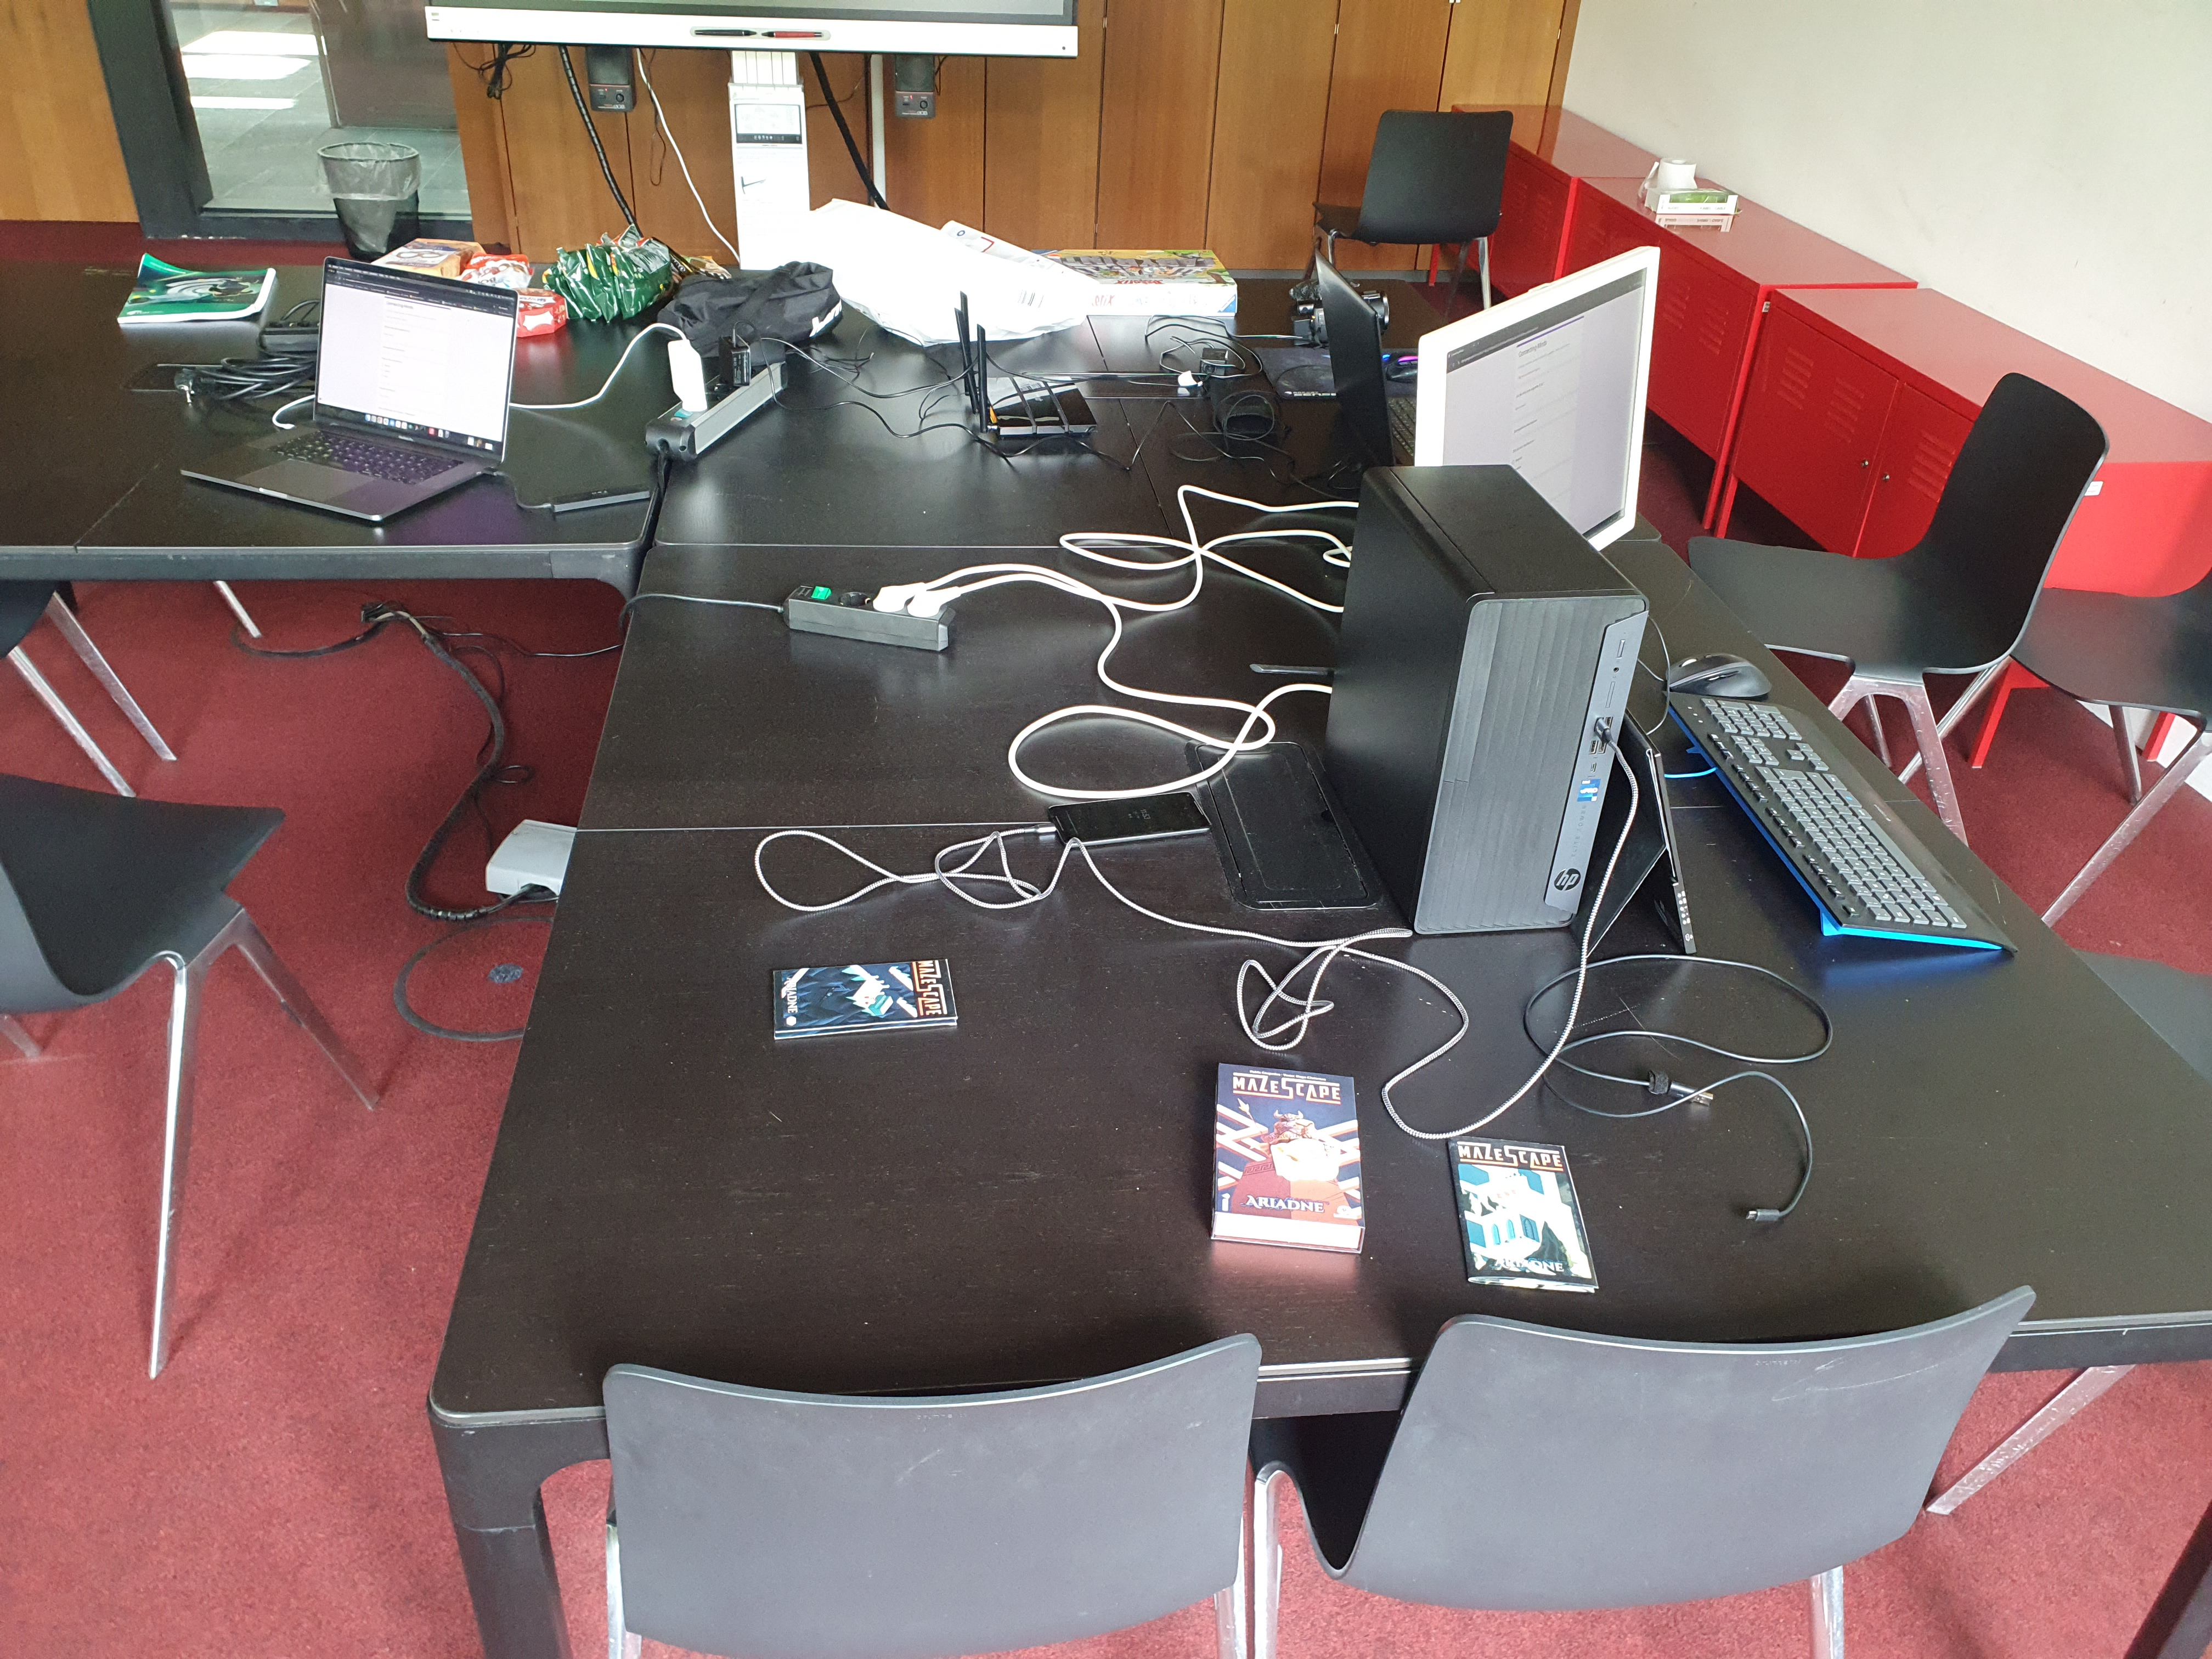
\includegraphics[width=0.8\linewidth]{content/pictures/Aufbau_00.jpg}
\caption{Versuchsaufbau des Experiments (Quelle: eigene Darstellung)}
\label{fig:study-experiment-00}
\end{figure}

\begin{figure}[ht]
\centering
\includegraphics[width=0.8\linewidth]{content/pictures/Aufbau_01.jpg}
\caption{Versuchsaufbau Seite des Players (Quelle: eigene Darstellung)}
\label{fig:study-experiment-01}
\end{figure}

\begin{figure}[ht]
\centering
\includegraphics[width=0.8\linewidth]{content/pictures/Aufbau_02.jpg}
\caption{Versuchsaufbau Seite des Watchers (Quelle: eigene Darstellung)}
\label{fig:study-experiment-02}
\end{figure}

Abbildung \ref{fig:study-experiment-00} zeigt die Anordnung des Seminarraums während der Versuchsdurchführung. Die beiden Spielteilnehmern saßen sich an einem quadratischen Tisch gegenüber. Zwischen ihnen war der Rechner für die Player-Anwendung positioniert, der zugleich als  physische Barriere diente. Diese räumliche Trennung war von zentraler Bedeutung, um zu verhindern, dass die Probanden in die Anwendung der jeweils anderen Person blicken und dadurch Aufgaben lösen konnten, ohne miteinander zu kommunizieren. Ein Blick in die Anwendung der anderen Person war ausdrücklich untersagt. 

Auf der rechten Seite des Tisches befand sich der Platz des Players (vgl. Abbildung \ref{fig:study-experiment-01}). Dieser steuerte seine Anwendung über einen Touchmonitor, der sich direkt vor ihm befand. Zusätzlich erhielt er für das Ausfüllen der Fragebögen im Rahmen der Versuchsdurchführung eine Tastatur sowie eine Maus und einen großen Bildschirm.

Der Watcher nahm auf der linken Seite des Tisches Platz (vgl. Abbildung \ref{fig:study-experiment-02}). Dort nutzte er das bereitgestellte Google Pixel, um die Watcher-Anwendung, die umgesetzte \ac{3D}-Anwendung zu bedienen. In diesem Bereich fanden auch der Vor- und Nachtest statt. Der 
Watcher konnte wählen, ob er sich im sitzen oder stehen durch das Labyrinth navigieren wollte.

Am linken Bildrand von Abbildung \ref{fig:study-experiment-00} ist ein weiterer Laptop zu sehen, über den der Watcher seine Fragebögen ausfüllte.

\section{Ergebnisse}

In diesem Kapitel werden die Ergebnisse der verschiedenen Fragebögen sowie der Videoaufzeichnung der Versuchsdurchführungen dargestellt. Die Präsentation der Ergebnisse erfolgt thematisch gegliedert in einzelnen Unterabschnitten, orientiert am jeweiligen inhaltlichen Schwerpunkt.

\subsection{Vorstellung der demographischen Daten}

An der Versuchsdurchführung nahmen insgesamt N = 14 freiwillige Probanden teil (3 weiblich, 11 männlich; M = 25,86; SD = 4,52 Jahre). Daraus ergaben sich sieben Dyaden für die Durchführung der Studie. Zwei Teilnehmer kannten sich zu Beginn der Untersuchung nicht bzw. lediglich flüchtig. 

Zwölf der Probanden gaben an, bereits Erfahrungen mit Video- und Computerspielen gesammelt zu haben; zwei Personen verfügten über keine diesbezüglichen Vorerfahrungen. Hinsichtlich der durchschnittlichen wöchentlichen Spielzeit ergab sich folgendes Bild: fünf Personen spielen mehr als 10 Stunden pro Woche, drei zwischen 6-10 Stunden, jeweils zwei zwischen 3-5 bzw. 1-2 Stunden und zwei gaben an, keine Zeit mit digitalen Spielen zu verbringen).

Bezüglich der Erfahrung mit Multiplayerspielen bestätigten 13 Teilnehmer entsprechende Vorerfahrungen, während eine Person angab, keine Multiplayer-Erfahrung zu haben. Drei Teilnehmer spielen mehr als 10 Stunden pro Woche Multiplayerspiele, eine Person zwischen 6-10 Stunden, vier zwischen 3-5 Stunden, fünf zwischen 1-2 Stunden und eine Person spielt keine Multiplayerspiele.

Die Spieltypenverteilung ergab, dass elf der Teilnehmer regelmäßig kompetitive Multiplayerspiele spielen, zehn kooperative, fünf kollaborative und eine Person eine andere Art von Spielen.

Zum Thema Touchsteuerung gaben 13 Personen an, bereits Erfahrung mit dieser Art der Bedienung gesammelt zu haben; eine Person verneinte dies. Eine Person nutzt Touchsteuerung häufig, drei gelegentlich und zehn selten.

Die Erhebung des Spielertyps auf Grundlage der Bartle-Typologie ergab, dass sich sieben Teilnehmer dem Typ Explorer zuordneten vier dem Typ Achiever, drei dem Typ Killer und keiner dem Typ Socializer.

\subsection{Vorstellung der Prototyp-Evaluation}

Die Darstellung der Fragebogenergebnisse erfolgt getrennt nach quantitativen und qualitativen Dimensionen.

Im Rahmen der quantitativen Auswertung der Fragebögen  \ac{SUS}, \ac{GEQ}, \ac{IMI} und \ac{NASA-TLX} wurde zunächst die deskriptiven Kennwerte \ac{M} und \ac{SD} berechnet. Diese Kennwerte wurden sowohl für die Gesamtstichprobe (N = 14) als auch getrennt für die Gruppen Player und Watcher ermittelt um potenzielle Unterschiede zwischen den beiden Anwendungsrollen identifizieren zu können.

Zur Prüfung signifikanter Gruppenunterschiede wurde im ersten Schritt die Verteilung der Daten auf Normalität untersucht. Diese Prüfung erfolgt einerseits visuell anhand von \ac{Q-Q}-Diagrammen und andererseits mithilfe des Shapiro-Wilk-Tests. Beide Verfahren wuirden getrennt f+r die Gruppen Player und Watcher durchgeführt.

Abhängig vom Ergebnis der Normalitätsprüfung kamen unterschiedliche statistische Verfahren zum Einsatz. Bei Vorliegen einer Normalverteilung in beiden Gruppen wurde ein zweiseitiger t-Test für unabhängige Strichproben durchgeführt. War in mindestens einer Gruppe keine Normalverteilung gegeben, wurde stattdessen der Mann-Whitney-U-Test als nichtparametrische Alternative angewendet.

Der folgende Abschnitt stellt die Ergebnisse dieser Auswertung für die einzelnen Fragebögen im Detail dar.

\paragraph{Quantitative Ergebnisse}

Der \ac{SUS} (Bewertungsskala von 1 = \say{stimme überhaupt nicht zu} bis 5 = \say{stimme voll und ganz zu}) ergab eine marginal hohe wahrgenommene Gebrauchstauglichkeit der Anwendungen (M = 69,11; SD = 13,64). Die Werte wieder dabei eine deutliche Streuung auf (Minimum = 47.5; Maximum = 92.5). Laut \citep[S. 36]{brooke_sus_2013} gilt ein \ac{SUS}-Wert von mindestens 73 als Schwelle für eine \say{gute} Gebrauchstauglichkeit. Die getrennte Betrachtung der Rollen ergab keine signifikanten Unterschiede zwischen der Watcher-Anwendung (M = 68,93; SD = 14,28) und der Player-Anwendung (M = 69,29; SD = 14,12); ein t-Test ergab  (p = 0,95; t = 2,29).

Für das In-Game-Modul des \ac{GEQ} (Bewertungsskala von 0 = \say{überhaupt nicht} bis 4 = \say{extrem}) zeigten die Mittelwerte, dass die Probanden insgesamt positive Spielerfahrungen machten. besonders hoch bewertet die Skalen \say{Positive Emotionen} (M = 3,07; SD = 0,83) und \say{Flow} ( M = 3; SD = 0,94). Auch \say{Kompetenzerleben} (M = 2,54; SD = 0,89), \say{Immersion} (p = 0,60; t = 2,24) und \say{Herausforderung} (M = 2,32; SD = 0,58) wurden tendenziell positiv bewertet. \say{Negative Emotionen} lagen überraschend niedrig (M = 0,54; SD = 0,75).

Die Vergleiche zwischen Player- und Watcher-Anwendung zeigten keine signifikanten Unterschiede. Für Kompetenz (p = 0,19; t = 2,18), Flow (p = 0,42; t = 2,21) sowie Immersion (p = 0,60; t = 2,24) ergaben sich durch die t-Test keine signifikanten Differenzen, ebenso wenig bei den übrigen Kategorien, für die aufgrund fehlender Normalverteilung der Mann-Whitney-U-Test herangezogen wurde (Anspannung: p = 0,65; U = 20,5; Herausforderung: p = 0,33; U = 17; negative Emotionen: p = 0,84; U = 22,5; positive Emotionen: p = 0,6; U = 20).

Auch im Abschnitt zur sozialen Präsenz des \ac{GEQ}, ebenfalls mit der Bewertungsskala von 0 bis 4, zeigten sich durchweg positive Bewertungen. Die Probanden berichteten, gegenseitiger Empathie empfunden zu haben (M = 3,11, SD = 0,55), verhielten sich aktiv beteiligt (M = 3,36; SD = 0,56) und zeigten nur wenige negative Gefühle (M = 1,26; SD = 0,57). Zwischen den Gruppen Player und Watcher ließen sich auch in diesem Teilbereich keine signifikanten Unterschiede feststellen (Empathie: p = 0,855; U = 22.5; Negative Gefühle: p = 0,14; t = 2,19; verhaltensbezogene Beteiligung: p = 0,45; t = 2,18).

Die Mittelwerte des Post-Game-Moduls des \say{GEQ}, ebenfalls mit der Bewertungsskala von 0 bis 4, zeigen, dass positive Erfahrungen auch nach dem Spielen des Prototyps im moderaten Ausmaß bestehen bleiben (M = 2,38; SD = 0,88). Gleichzeitig fiel die Rückkehr in die Realität den Teilnehmern vergleichsweise leicht (M = 1,02; SD = 0,69). Geringe negative Erfahrungen (M = 0,31; SD = 0,31) deuten darauf hin, dass etwaiger Frust durch Gebrauchstaugliche-Probleme nicht nachwirken. Auch das Maß an empfundenem Erschöpfungszustand war niedrig (p = 0,88; t = 2,18), was darauf hinweist, dass doe Probanden durch den Prototyp nicht übermäßig über einen längeren Zeitraum hinweg ermüdet wurden.

In den Einzelkategorien \say{Positiven Erfahrungen} p = 0,56; t = 2.18), \say{Negative Erfahrungen} (p = 0,3: U = 16) und \say{Müdigkeit} (p = 0,88; t = 2,18) konnten keine signifikanten Unterschiede zwischen den beiden Anwendungen festgestellt werden. Lediglich in der Kategorie \say{Rückkehr in die Realität} wurde ein signifikanter Unterschied beobachtet (p = 0,04; U = 8.5). Die Anwendungen der Watcher-Rolle wurde mit einem Mittelwert von M = 1,43 höher bewertet als jene des Players (M = 0,62). Obwohl die absolute Ausprägung des Wertes moderat ist, deutet dieses Ergebnis darauf hin, dass die Watcher-Anwendung, vermutlich aufgrund ihrer Funktion und der ihr zugeschriebenen Steuerungs- bzw. Führungsrolle, anders wahrgenommen wurde als die Player-Anwendung.

Die Ergebnisse der Skala Interesse/Vergnügen des \ac{IMI} (Bewertungsskala von 1 = \say{trifft überhaupt nicht zu } bis 4 = \say{trifft völlig zu}, zeigen ein insgesamt hohes Maß an Interesse und Vergnügen (M = 3,60; SD = 1,38). auch hier ergaben sich keine signifikanten Unterschiede zwischen den Rollen Player und Watcher (p = 0,45; t = 2,21). 

Die Ergebnisse des \ac{NASA-TLX} (Ursprünglich 0-10, hier skaliert auf eine 100-Punkte-Skala) verdeutlichen, dass die gestellten Rätsel sowie die Steuerung insbesondere eine erhöhte geistige Anstrengung erforderten (M = 63,57; SD = 14,47). Im Gegensatz dazu war die körperliche Belastung sehr gering  (M = 4,29; SD = 6,46), ebenso die zeitliche Beanspruchung (M = 28,57; SD = 16,57). Der Leistungsstil des Fragebogens (M = 75,14; SD = 17,85) belegt, dass der Prototyp durchgängig erfolgreich absolviert wurde. Die wahrgenommene Anstrengung wurde als moderat beschrieben (M = 50,71; SD = 19,79) , während die Frustration vergleichsweise niedrig ausfiel  (M = 29,29; SD = 31). Die Ergebnisse legen nahe, dass die Rätsel und Steuerung insgesamt fordernd, aber nicht überfordernd gestaltet waren. Gleichwohl lassen sich Hinweise auf verbesserungswürdige Gebrauchstauglichkeit im gemessenen Frustrationsniveau erkennen.

Zwischen den Rollen Player und Watcher konnten in keiner der \ac{NASA-TLX}-Unterkategorien signifikante Unterschiede festgestellt werden (Geistige Anforderungen: p = 0,86; t = 2,22; Körperliche Anforderungen: p = 0,55; U = 29; Zeitliche Anforderungen: p = 0,76; t = 2,23; Leistung: p = 0,78; t = 2,21; Anstrengung: p = 0,9; t = 2,19; Frustration: p = 0,85; U: 26,5).

Für die qualitative Auswertung der offenen Rückmeldungen im Freitextfeld \say{Welches sonstige Feedback hast du?} wurde wie in Kapitel \ref{sec:pre-study-method-results} das Verfahren der thematischen Analyse nach \cite{braun_using_2006} herangezogen.

\paragraph{Qualitative Ergebnisse}

Abbildung \ref{fig:qualitative-results} zeigt, dass die Antworten im Freitextfeld des Fragebogens in fünf inhaltliche Kategorien eingeordnet werden konnten. Diese lassen sich grob in zwei übergeordnete Bereiche Gliedern: konstruktive Kritik an den Anwendungen sowie allgemeines positives Feedback zum Spielkonzept und zur Durchführung der Studie. Der zentrale Aspekt der konstruktiven Rückmeldung betrifft insbesondere die verbesserungswürdige Steuerung, wobei vor allem die Steuerung der Watcher-Rolle kritisch reflektiert wurde. Positiv hervorgehoben wurden hingegen das Rätseldesign sowie die Gestaltung der Spielumgebung.

\begin{figure}[ht]
\centering
\includegraphics[width=1\linewidth]{content/pictures/Qualitative-Auswertung-Schritt-1.png}
\caption{Ergebnis der groben Kategorisierung nach \cite{braun_using_2006} (Quelle: eigene Darstellung)}
\label{fig:qualitative-results}
\end{figure}

Abbildung \ref{fig:qualitative-results-end} fasst die zentralen Rückmeldungen der Teilnehmer zusammen. Die Steuerung, insbesondere in der Watcher-Anwendung, wurde insgesamt als problematisch bewertet. Mehrere Kommentare beschrieben sie als umständlich, unintuitiv, träge (\say{unresponsiv}) oder \say{clunky} sowie als insgesamt unklar. Besonders betroffen waren dabei die Yaw- und Zoom-Gesten der \ac{3D}-Anwendung. Als mögliche Verbesserung wurde unter anderem die Integration unterstützender Elemente in das Overlay-\ac{UI} angeregt, um eine bessere Differenzierung zwischen der Zoom- und der Rotationsfunktion der Ansicht zu ermöglichen.

In der Player-Anwendung wurde das Fehlen einer vertikalen Kamerabewegung in der First-Person-Ansicht kritisiert, da derzeit nur eine fixe vertikale Perspektive genutzt werden kann. Zudem kam es mehrfach zu Schwierigkeiten bei der Auswahl einer Zielposition, zu der sich der Avatar bewegen sollte.

Hinsichtlich des Rätsel- und Umgebungsdesign wurde angemerkt, dass die Lösungsfindung teilweise noch unausgereift und zu herausfordernd sei. Es wurde vorgeschlagen, zusätzliche Hinweise in die Spielwelt zu integrieren, um die Rätsel zugänglicher zu gestalten. Weiterhin wurde empfohlen, bereits gelöste Räume zu deaktivieren, da diese andernfalls bei der Lösung neuer Aufgaben als irritierende Störfaktoren wahrgenommen werden. 

Die Nutzerstudie wurde insgesamt als interessant und professionell umgesetzt bewertet. Gleichwohl wurde der Vor- und Nachtest mit MazeScape vereinzelt als frustrierend empfunden.

Insgesamt wurde der Spielprototyp als unterhaltsam wahrgenommen. Das Spielkonzept von Connecting-Minds wurde als überzeugen und ansprechend umgesetzt bewertet. Positiv hervorgehoben wurde außerdem das einfache Setup.

\begin{figure}[ht]
\centering
\includegraphics[width=1\linewidth]{content/pictures/Qualitative-Auswertung-Schritt-2.png}
\caption{Ergebnis der feinen Kategorisierung nach \cite{braun_using_2006} (Quelle: eigene Darstellung)}
\label{fig:qualitative-results-end}
\end{figure}

\subsection{Einordnung der qualitativen und quantitativen Ergebnisse}

Die Auswertung des Freitextfeldes liefert differenzierte Hinweise auf die Ursachen für den vergleichsweise niedrigen Wert im \ac{SUS}. Die eingeschränkte Gebrauchstauglichkeit lässt sich vor allem auf mangelnde Klarheit sowie aif die verbesserungswürdige Umsetzung der Steuerung in beiden Anwendungen, insbesondere jedoch in der Watcher-Anwendung, zurückführen. Darüber hinaus fließen aich die im Freitextfeld thematisierten Kritikpunkte am Rätsel- und Umgebungsdesign in die Bewertung ein.

Der durchschnittliche Frustrationswert im \ac{NASA-TLX} (M = 29,29) kann diese Einschätzungen nur teilweise stützen. Zwar liegt der Mittelwert im unteren Bereich, die hohe Standardabweichung von SD = 31 weist jedoch darauf hin, dass einzelne Teilnehmer ein deutlich höheres Maß an Frustration erlebten.

Demgegenüber zeigen die Ergebnisse des \ac{IMI} und des \ac{GEQ}, unterstützt durch das positive qualitative Feedback, dass die Probanden trotz der genannten Herausforderungen Interesse, Freude und Spielspaß entwickeln konnten.

\subsection{Vorstellung der Ergebnisse der subjektiven Wahrnehmung der Probanden}

Im Folgenden werden die Ergebnisse zur subjektiven Wahrnehmung der Probanden im Hinblick auf den \ac{IOS} sowie den \ac{SAM} dargestellt. Die Einschätzungen wurden zu zwei Messzeitpunkten erhoben. Einmal vor dem Vortest als \say{Ground Truth} und erneut nach dem Nachtest, um potenzielle Veränderungen im Erleben sozialer Nähe und affektiver Zustände im Verlauf des Experiments sichtbar zu machen.

\begin{figure}[ht]
\centering
\includegraphics[width=1\linewidth]{content/pictures/IOS_SAM_Overal.png}
\caption{Ergebnisse des \ac{IOS} und \ac{SAM} auf alle Probanden bezogen (Quelle: eigene Darstellung)}
\label{fig:ios_sam_overal}
\end{figure}

Abbildung \ref{fig:ios_sam_overal} zeigt die aggregierten Ergebnisse der Erhebungen mittels \ac{IOS} und \ac{SAM}. Der analysierte Datensatz umfasst sowohl die Einschätzungen der Player- als auch Watcher. Eine differenzierte Betrachtung der Entwicklung innerhalb der einzelnen Rollen erfolgt im Anschluss in Abbildung \ref{fig:ios_sam_roles}.

Zur Vorbereitung der statistischen Auswertung wurde zunächst geprüft, ob die Daten eine Normalverteilung ausweisen. Für den Gesamtdatensatz erfolgt diese Überprüfung mittels Kolmogorov-Smirnov-Test. Die Teilstichproben wurden, analog zur Auswertung der Fragebögen zum Prototyp, zunächst visuell über \ac{Q-Q}-Plots begutachtet und anschließend mit dem Shapiro-Wilk-Test auf Normalverteilung getestet.

Lagen die Vor- und Nachtest-Daten normalverteilt vor, wurde ein t-Test für abhängige Stichproben durchgeführt, um mögliche signifikanten Veränderungen festzustellen. Zusätzlich wurde die Effektstärke berechnet. Für nicht-normalverteilte Daten wurde stattdessen der Wilcoxon-Test für abhängige Stichproben angewendet.

Zur Analyse der Differenzen zwischen den beiden Rollen wurde untersucht, welche Gruppe im Verlauf des Experiments stärkere Veränderungen aufwies. Für normalverteilte Subgruppen kam der Welch-Test zur Anwendung, bei nicht-normalverteilten Verteilungen wirde der Mann-Whitney-U-Test eingesetzt.

\paragraph{Allgemeine Auswertung}

Zunächst zeigt sich, dass die empfundene soziale Nähe innerhalb der Dyaden, gemessen über den \ac{IOS}, im Mittelwert signifikant ansteigt. Dieser Veränderung deutet darauf hin, dass sich die subjektive wahrgenommene soziale Nähe der Teilnehmenden im Verlauf des Experiments erhöht hat. Die zugehörige Effektstärke weist auf eine mittlere Korrelation hin.

Bezüglich der Valenz, also der affektiven Bewertung im Sinne positiver und negativer Emotionen (Bewertungsskala von 1 = \say{glücklich} bis 9 = \say{unglücklich}), zeigt sich im Mittelwert ein minimal Anstieg. Die Probanden konnten sich als ziemlich glücklich einschätzen. Die Veränderung ist jedoch statistisch nicht signifikant und weis lediglich eine sehr geringe Korrelation auf.

Auch die Erregung bzw. Aktivierung der Teilnehmer (Activation, Bewertungsskala von 1 = \say{aufgeregt} bis 9 = \say{entspannt}) steigt im Mittelwert leicht an. Insgesamt sind die Probanden zum Vortest und Nachtest recht entspannt aufgetreten. Die Beobachtete Veränderung ist zu gering, dass sie signifikant sein kann. Außerdem weißt sie keine Korrelation auf.

Im Bereich der wahrgenommenen Dominanz (Control, Bewertungsskala von 1 = \say{fremdkontrolliert} bis 9 = \say{vollständig in Kontrolle}), zeigt sich ein höherer Anstieg des Mittelwerts als bei den zuvor gemessen Skalen. Sie zeigten eine ausgeglichene Dominanz. Auch diese Veränderung ist statistisch nicht signifikant und geht mit einer nur geringen Korrelation einher.

\paragraph{Auswertung in der Unterscheidung zwischen Player und Watcher}

\begin{figure}[ht]
\centering
\includegraphics[width=1\linewidth]{content/pictures/IOS_SAM_Player_Watcher.png}
\caption{Ergebnisse des \ac{IOS} und \ac{SAM} auf beide Spielerrollen bezogen (Quelle: eigene Darstellung)}
\label{fig:ios_sam_roles}
\end{figure}

Der vollständige Datensatz wurde im Anschluss in die zwei Untergruppen Player und Watcher unterteilt und getrennt analysiert.. Dabei zeigt sich, dass der signifikante Anstieg in der Entwicklung der sozialen Nähe ausschließlich bei den Teilnehmern der Player-Rolle festzustellen ist. In dieser Gruppe fällt auch die Korrelation höher aus als in der Watcher-Gruppe. zwischen den beiden Gruppen konnte jedoch kein signifikanter Unterschied in der Veränderung der sozialen Nähe festgestellt werden.

In Übereinstimmung mit den Ergebnissen der Gesamtstichprobe zeigen sich auch in dem Subgruppen keine signifikanten Veränderungen in den Dimensionen Valenz, Activation und Control.

\subsection{Vorstellung der Ergebnisse der Quantisierung der Gesprächsflüsse}

In diesem Abschnitt werden die Ergebnisse der durchgeführten Vor- und Nachtests des Versuchsaufbaus dargestellt. Die Tests wurden jeweils pro Dyade aufgezeichnet und anschließend mithilfe von \say{whisperx} transkribiert (vgl. \citealp{bain_whisperx_2023}). Die Vorgehensweise zur Analyse der Transkripte orientierte sich an der Methode von \cite{nasir_effect_2015}, welche ein strukturiertes Verfahren zur quantitativen Auswertung vorgibt.

Zunächst wurden die Transkripte in einzelne Gesprächsblöcke unterteilt, die sich entweder durch längere Pausen oder durch einen thematischen Wechsel im Gesprächsverlauf voneinander abgrenzen ließen. Analog zur Definition bei \citeauthor{nasir_effect_2015} wurde eine Pause als ununterbrochener Zeitraum von mehr als drei Sekunden definiert, in dem keiner der Probanden spricht oder kommuniziert, ausgenommenen kurze Interjektionen.

Zur qualitativen Analyse des Gesprächsverlaufs wurden die Kommunikationsblöcke in sog.  \say{Floor Holding}-Muster unterteilt (vgl. \citealp{edelsky_whos_1981}). Floor Holding beschreibt dabei Situationen, in denen eine Person oder eine Gruppe von Personen den Gesprächsfluss für einen bestimmten Zeitraum dominiert (vgl. \citealp[S. 135]{nasir_effect_2015}). In Anlehnung darauf wird zwischen \say{\ac{CF}} und  \say{\ac{SF}} unterschieden. Während beim \ac{CF} beide Probanden aktiv am Gespräch teilnehmen und den Gesprächsverlauf gemeinsam gestalten, dominiert beim \ac{SF} nur eine Person das Gespräch, während die andere lediglich reagiert oder kurze Antworten gibt.

Darüber hinaus wurden die Gesprächsblöcke zeitlich codiert, um Beginn und Dauer innerhalb der Videoaufzeichnung präzise zu erfassen. So konnte bestimmt werden, wie lange die Gespräch jeweils andauerten und welchen relativen Anteil sie an der gemeinsamen Arbeitszeit des jeweiligen Tests einnahmen. Zusätzlich wurde, analog zur Methodik von \citeauthor{nasir_effect_2015}, die Anzahl der \say{Turns} gezählt, wobei ein Turn jeweils ein einzelner Redebeitrag eines Probanden darstellt. Ergänzend wurden auch die Wortzahlen pro Abschnitt erfasst, um diese später für Vergleiche zwischen den Teilnehmern und zwischen Vor- und Nachtest herziehen zu können.

Abschließend wurde die Gesamtzahl der gesprochenen Wörter pro Teilnehmer im jeweiligen Testdurchlauf erfasst. Diese wurde in Relation zur Gesamtwortanzahl des jeweiligen Tests gesetzt, um den individuellen Gesprächsanteil innerhalb der Dyade zu bestimmen.

Ergänzend zur Methodik von \citeauthor{nasir_effect_2015} wurde zusätzlich erhoben, welcher der beiden Probanden wie häufig Gesprächsblöcke initiierte. Dieser Indikator dient der Bewertung der Entwicklung kommunikativer Initiative im Verlauf des Experiments.

Zur statistischen Auswertung wurden die jeweiligen Stichproben zunächst mithilfe des Shapiro-Wilk-Tests auf Normalverteilung geprüft. Bei normalverteilten Stichproben wurden Veränderungen zwischen Vor- und Nachtest mittel t-Test für abhängige Stichproben zum Einsatz. Für den Vergleich unabhängiger Stichproben wurde der Welch-Test verwendet.

\begin{figure}[ht]
\centering
\includegraphics[width=1\linewidth]{content/pictures/quantitative_communication_results.png}
\caption{Ergebnisse des quantitativen Kommunikationsverhaltens aller Gruppen im Vergleich Vortest/Nachtest (Quelle: eigene Darstellung)}
\caption*{\footnotesize Das Kürzel (n) bezeichnet normalisierte Werte auf 10 Minuten Gesprächsdauer.}
\label{fig:communication-results}
\end{figure}

Abbildung \ref{fig:communication-results} zeigt die Ergebnisse der quantitativen Untersuchung der einzelnen Probandentests. Abweichend von Nasir, der eine testweise Auswertung vornimmt, wurde hier pro Merkmal der durchschnittliche Wert aus allen sieben Tests für den Vor- und Nachtest verwendet.

Die einzelnen Gruppen erhielten für das kooperative Lösen der Labyrinth-Aufgabe 10 Minuten Zeit. Jedoch waren einige Gruppen früher fertig, manche wiederum wurden gar nicht fertig (M = 08:05 Minuten; SD = 02:27 Minuten Bearbeitungszeit im Vortest (M = 06:56 Minuten; SD = 03:15 Minuten Bearbeitungszeit im Nachtest). Aus diesem Grund wurden die in Abbildung \ref{fig:communication-results} betreffenden Merkmale normalisiert.

Die durchschnittlich gesprochene Wörteranzahl sinkt in der Entwicklung vom Vor- zum Nachtest leicht. Dieses negative Veränderung ist jedoch nicht signifikant und besitzt auch nur eine sehr kleine negative Korrelation. Außerdem stieg die bereits im Vortest hohe Standardabweichung ein Stück weiter an, wodurch eine größere Streuung der Daten aus den Einzelgruppen sichtbar wird. 

Die Wörterbeiträge der Probanden aus den jeweiligen Gruppen des Players und Watchers wurden jeweils in ihren Tests im Verhältnis zu den gesamt gesprochenen Wörtern betrachtet. Der Mittelwert der Wortbeteiligungen der Player sank im Nachtest leicht, wohingegen die Wortbeteiligungen der Watcher leicht anstiegen. Beide Änderungen sind nicht Signifikant und besitzen auch nur eine geringe Korrelation. Die Anzahl der gemessenen \say{Turns} steigt jedoch leicht, um ein nicht signifikantes Maß an.

Die Anzahl und die Länge der Pausen innerhalb des Gesprächsprotokolls reduzierten sich im Nachtest. In diesem Testszenario ist diese Veränderung zwar nicht signifikant, allerdings kann die mittlere negative Korrelation darauf hinweisen, dass in einem längeren Szenario Pausenzeiten signifikant reduziert werden könnten. Eine Reduktion der Anzahl und der Länge der Pausen kann zu einem positiven Kommunikationsverhalten führen.

Eine Analyse des Floor Holding Verhaltens der jeweiligen Probanden-Paare zeigt, dass das Kollaborative Verhalten im Mittelwert minimal ansteigt, jedoch in den \ac{SF}s der jeweiligen Teilnehmer im Vergleich stärker ansteigt. Alle drei Änderungen haben keine signifikante Verbesserung, auch eine niedrige Korrelation weißt nicht darauf hin, dass mit einem längeren Szenario und einer größeren Stichprobe am Wachstum eine Verbesserung messbar wird.

Die Auswertung der Gesprächsstarts zeigte, dass die Probanden, die die Player Anwendung gespielt haben, im Nachtest seltener die Initiative ergriffen als noch im Vortest. Bei den Probanden der Watcher Anwendung ist es umgekehrt. Sie zeigten im Nachtest eine höhere Initiative und begannen öfters mit den Gesprächssequenzen. Beide Änderungen sind zwar nicht signifikant, besitzen aber eine mittlere Korrelation. Beim Vergleich der beiden Untergruppen konnte ein signifikanter Unterschied festgestellt werden. Bei einer größeren Stichprobe könnten die Entwicklungen der Initiativen signifikant werden.

In der gemeinsamen Gesprächsführung konnten sich die Probanden nicht verbessern, allerdings konnten sie häufiger von sich aus den Gesprächsfluss dominieren, wodurch ihr Selbstbewusstsein etwas beitragen zu können, gestärkt werden konnte. Allerdings konnten in dieser Bewertungsform keine signifikanten Unterschiede festgestellt werden.


\subsection{Vorstellung der Ergebnisse zum Thema Leadership}
In diesem Abschnitt werden die Ergebnisse des Leadership-Fragebogens von \cite{emmerich_game_2016} in Bezug auf die Ergebnisse der quantitativen Auswertung der Vor- und Nachtests vorgestellt.

Zunächst wurden für jeden Probanden der Mittelwert der gewählten Werte berechnet (Wertung von 1 = trifft nicht zu; bis 5 = trifft vollkommen zu). Anschließend erfolgt die Gesamt-Durchschnittsberechnung. Die teilgenommenen Probanden zeigten insgesamt ein mittleres Maß an Führung (M = 3.92; SD = 1.18). 

Um die Mittelwerte der Player und Watcher Untergruppen miteinander vergleichen zu können, wurde zunächst durch den Shapiro-Wilk-Test auf Normalverteilung überprüft. Der Vergleich der Mittelwerte erfolgt über den ungepaarten t-Test.

Zwischen den Probanden der Watcher-Gruppe (M = 3.06; SD = 1.24) und der Player-Gruppe (M = 2.99; SD = 1.14) konnte kein signifikanter Unterschied festgestellt werden (p = 0.71; t = 2.18). 

Im Anschluss wurde untersucht, ob das Leadership Verhalten der einzelnen Probanden eine mögliche Korrelation mit ihren gesprochenen Worten im Nachtest besteht. Dafür wurde der Spearman'sche Rangkorrelationskoeffizient verwendet.

\begin{figure}[ht]
\centering
\includegraphics[width=1\linewidth]{content/pictures/Korrelation_Leadership_Wordcount_full.png}
\caption{Korrelation des Leaderships mit den gesprochenen Worten aus der quantitativen Gesprächsauswertung}
\label{fig:correlation_leadership_wordcount}
\end{figure}

In Betrachtung aller Probanden mit ihrem durchschnittlichen Leadership-Wert konnte nur eine sehr schwache Korrelation und keine Signifikanz festgestellt werden (rs(14) = 0.13; p = 0.66) (vgl. Abbildung \ref{fig:correlation_leadership_wordcount}, linkes Schaubild). In der Untergruppe der Watcher (vgl. Abbildung \ref{fig:correlation_leadership_wordcount}, rechtes Schaubild) konnte eine mittlere Korrelation festgestellt werden, welche ebenfalls nicht signifikant ist (rs(7) = 0.46; p = 0.29). In der Untergruppe der Player konnte keine Korrelation festgestellt werden (vgl. Abbildung \ref{fig:correlation_leadership_wordcount}, mittleres Schaubild). Diese ist ebenfalls nicht signifikant (rs(7) = 0; p = 1)

Da in dieser Arbeit eine verbesserte Kommunikation zwischen den Probanden angestrebt wird, steht insbesondere die Förderung kollaborativer Kommunikationsanteile im Fokus. Wie in der quantitativen Auswertung bereits festgestellt werden konnte, gab es keine signifikante Änderung in den Anteilen des \ac{CF}s. Da die Mittelwerte der Leadership-Selbsteinschätzung im mittleren Bereich liegen, lässt vermuten, dass keiner der teilnehmenden Personen eine dominante Führungsrolle einnimmt. Stattdessen könnte dies auf ein grundsätzlich kooperatives Miteinander hinweisen, in dem Führungsaspekte gleichmäßig verteilt und kollaborative Kommunikationsformen bevorzugt werden.

Dafür wurden nun Durchschnitte der Leadership-Werte der Probanden genommen, die an den Tests gemeinsam teilgenommen haben. Diese werden nun mit den Einzelwerten der \ac{CF}s der eigenen Tests verglichen.

\begin{figure}[ht]
\centering
\includegraphics[width=1\linewidth]{content/pictures/korrelation_leadership_cfh.png}
\caption{Korrelation des Leaderships pro Probanden-Paar mit dem \ac{CF}-Anteil ihres Nachtests}
\label{fig:correlation_leadership_cfh}
\end{figure}

Es konnte keine Korrelation (vgl. Abbildung \ref{fig:correlation_leadership_cfh}) zwischen dem durchschnittlichen subjektiven Leadership Empfinden der Probanden-Paare mit ihrem \ac{CF}-Anteil in ihren jeweiligen Nachtests festgestellt werden. Diese hat außerdem keine Signifikanz (rs(7) = -0.08; p = 0.86).

Zuletzt wurde noch das subjektive Empfinden des Leaderships mit den gemessenen Anteilen der Gesprächsstarts untersucht (vgl. Abbildung \ref{fig:correlation_leadership_conversation_starts}). Auch hier zeigten sich weder in der Gruppe der Player (rs(7) = -0.07; p = 0.88), noch in der Gruppe der Watcher (rs(7) = -0.03; p = 0.94) Korrelationen, die ebenfalls nicht signifikant sind. 

\begin{figure}[ht]
\centering
\includegraphics[width=1\linewidth]{content/pictures/Korrelation_Leaderhip_Start_of_conversation.png}
\caption{Korrelation des Leaderships von Player und Watchern mit dem Anteil der Konversationsstarts}
\label{fig:correlation_leadership_conversation_starts}
\end{figure}

Insgesamt zeigt sich, dass das mittlere empfundene Leadership keine Auswirkung auf die Entwicklungen innerhalb der quantitativen Untersuchung hat.

\subsection{Vorstellung der Ergebnisse zum Thema Kognitive Empathie}
In diesem Unterkapitel wird das Ergebnis des Fragebogens zur Kognitiven und Affektiven Empathie vorgestellt (Skala von 1 = Stimme überhaupt nicht zu bis 5 = Stimme voll und ganz zu). Hierbei wurden die Einzelwertungen der beiden Fragebögen zur Kognitiven Empathie ausgezählt und zusammengerechnet. Das Gesamtergebnis zeigt, dass die Probanden ein hohes Maß an kognitiver Empathie zeigen (M = 70; SD = 10.21; Maximal Wert 95). 

Ein ungepaarter t-Test-Vergleich bei ungleichen Varianzen zwischen den Probanden der Player (M = 68.71; SD = 9.96) und Watcher (M = 71.29; SD = 11.09) Untergruppe konnte kein signifikanter Unterschied festgestellt werden, obwohl die Wertung der Watcher leicht höher ist, als die der Player. 

Über den Spearman'sche Rangkorrelationskoeffizienten wurde überprüft, ob das hohe Maß an kognitiver Empathie einen Einfluss auf den hohen Anteil an \ac{CF} im Nachtest hat. 

\begin{figure}[ht]
\centering
\includegraphics[width=1\linewidth]{content/pictures/Korrelation_Kognitive_Empathie_cfh.png}
\caption{Korrelation kognitiver Empathie mit \ac{CF}-Anteil pro Probanden-Paar}
\label{fig:correlation_kognitive_empathy_cfh}
\end{figure}

Es besteht keine Korrelation (vgl. Abbildung \ref{fig:correlation_kognitive_empathy_cfh}) zwischen der Kognitiven Empathie und dem \ac{CF}-Anteil des Nachtests ((rs(7) = -0.04; p = 0.94).



\subsection{Vorstellung der Ergebnisse zum Thema Fragen zum Nutzen eines spielerischen Ansatzes und Verbesserung der Kommunikation, insbesondere auch im Umgang mit nicht bekannten Personen}
(Anmerkung: Nach Sammlung der Ergebnisse wurde festgestellt, dass die Fragebogen-Antworten von einem Probanden nicht abgespeichert oder abgeschickt wurde. Aus diesem Grund werden hier nur von N = 13 Probanden die Antworten ausgewertet.)

Abschließend werden nun die Ergebnisse vom letzten Fragebogen zum Thema \say{Fragen zum Nutzen eines spielerischen Ansatzes und Verbesserung der Kommunikation, insbesondere auch im Umgang mit nicht bekannten Personen} vorgestellt. Für dieses Thema existiert bislang kein standardisierter Fragebogen. Der für dieses Thema entworfene Fragebogen (Wertung von 1 = Stimme trifft überhaupt nicht zu bis 5 = Stimme trifft voll und ganz zu) umfasst folgende Fragen:
\begin{enumerate}
    \item Spielerische Elemente erleichtern es mir, mit anderen Personen in Kontakt zu treten.
    \item Der Einsatz von Spielelementen (z. B. Aufgaben, Belohnungen, Avatare) kann die Kommunikation zwischen unbekannten Personen fördern.
    \item Ich bin offen dafür, neue Menschen kennenzulernen.
    \item Interaktive oder spielerische Funktionen in digitalen Anwendungen erleichtern mir den Austausch mit anderen.
    \item Ich würde eine digitale Plattform nutzen, die durch spielerische Elemente den Kontakt zu mir unbekannten Personen erleichtert.
    \item Es fällt mir leichter, mit anderen Personen in Kontakt zu treten, wenn spielerische Komponenten involviert sind.
    \item Ich erkenne einen Mehrwert darin, spielerische Kommunikation in beruflichen oder sozialen Kontexten zu integrieren.
\end{enumerate}

Die Fragen 1,2,4 und 6 können dabei in die Kategorie \say{Gamification erleichtert soziale Interaktion} eingeteilt werden. Die Frage 5 umfasst die Kategorie \say{Akzeptanz / Nutzungsintention gamifizierter Plattformen}. Die Fragen 3 und 7 bilden die Kategorie der \say{sozialen Offenheit und Haltung zu spielerischer Kommunikation}.

Beim Thema \say{Gamifikation erleichtert soziale Interaktion} zeigen die Ergebnisse der Probanden ein hohes Maß an Zustimmung (M = 4.42: SD = 0.61). Zum Thema \say{Akzeptanz / Nutzungsintention gamifizierter Plattformen} zeigt sich ein eher wechselhaftes Gesamtbild (M = 3.5; SD = 1.27). Allerdings zeigen sie eher eine soziale Offenheit und Haltung gegenüber spielerischer Kommunikation (M = 3.77; SD = 0.95).

\section{Hypothesenüberprüfung}
Aufgrund des Umfangs des Forschungshintergrundes und des Versuchsaufbaus wurden im Vorfeld der Nutzerstudie die Anzahl der zu überprüfenden Hypothesen auf fünf festgelegt.

Wie im Kapitel der Analysen der artverwandten Spiele, wurden zunächst Hypothesen, die vor der Durchführung der Nutzerstudie formuliert wurden, mit den dokumentierten Ergebnissen verglichen. 

Die Ergebnisse der ausgewerteten Fragebögen und Transkripte zeigen, dass mit Connecting-Minds ein spannendes Spiel konzipiert und umgesetzt werden konnte, das durch seine Spielmechanik eine interessante Erfahrung bieten konnte. Allerdings konnte keine gute gebrauchstaugliche Steuerung in die Anwendungen eingebaut werden, wodurch das Spielerlebnis und die Wirkung des Prototyps gemindert wurde. Allerdings konnte beobachtet und festgestellt werden, dass die soziale Nähe der Probanden gestiegen ist und der Prototyp auf diese Weise eine positive Auswirkung hat. Aufgrund der niedrigen Teilnehmerzahl der Nutzerstudie konnten keine signifikanten Veränderungen im Kommunikationsverhalten festgestellt werden, wodurch die Kernwirkung des Prototyps nicht bestätigt werden konnte. Jedoch kann die Anwendung dazu beitragen, dass die Hemmschwelle für das Kennenlernen von für sich fremden Personen sinkt.

\begin{figure}[ht]
\centering
\includegraphics[width=1\linewidth]{content/pictures/Hypothesen_Nutzerstudie.PNG}
\caption{Hypothesenüberprüfung der Nutzerstudie}
\label{fig:hypothesis_user_study}
\end{figure}

\section{Handlungsempfehlungen}
Auf Basis der erhaltenen Ergebnisse der quantitativen und qualitativen Datenerhebung wurden nun Handlungsempfehlungen formuliert, welche auf Basis des Severity Rankings priorisiert werden (vgl. Abbildung \ref{fig:call_to_actions_user_study}).

\begin{figure}[ht]
\centering
\includegraphics[width=1\linewidth]{content/pictures/Handlungsempfehlung_Nutzerstudie.png}
\caption{Handlungsempfehlungen zur Nutzerstudie}
\label{fig:call_to_actions_user_study}
\end{figure}

Das Hauptaugenmerk auf die Weiterentwicklung der Anwendungen von Connecting-Minds muss auf der Überarbeitung der Steuerung liegen. Nahezu alle Probanden der Watcher-Anwendung bemängelten die Steuerung der 3D-Anwendung. Insbesondere eine Unterschiedung oder feinere Abgrenzung zwischen der Yaw- und Zoom-Geste ist in der Watcher-Anwendung gewünscht. Außerdem waren manche Rätsel innerhalb des Prototyps nicht final durchdacht und benötigen außerdem weitere konzeptionelle Iterationen, die Anhand der Umsetzung evaluiert werden sollten. 
Sollte es eine zukünftige Forschung in dem Themenbereich dieser Arbeit geben, sollten zu weiteren Zeitpunkten innerhalb der Nutzerstudie Daten erhoben werden, um genaue Entwicklungen innerhalb der Daten feststellen zu können. Darunter zählt bspw. der \ac{IOS}, der sowohl vor und nach dem Vortest, nach dem Prototyp und nach dem Nachtest ausgefüllt werden könnte. Analog dazu verhält es sich bei den Fragebögen zum Thema Leadership und kognitiver Empathie. 
Zusätzlich zur quantitativen Auswertung der Transkripte könnte eine quantitative Auswertung erfolgen, wodurch die Entwicklung der Art und Weise des Kommunikationsverhalten zusätzlich noch untersucht werden kann. Zuletzt konnten aufgrund des Umfangs des Projekts und der Studie nicht alle Aspekte des Spiels konzipiert und umgesetzt werden, wodurch bspw. an vielen Stellen das \ac{UI} unvollständig ist und oft nur erste Skizzen enthält.

\section{Zusammenfassung und Interpretation der Ergebnisse}
Nach der Auswertung der Fragebögen zum Prototyp zeigte sich, dass im Vorfeld der großen Nutzerstudie noch mehr Zwischentests mit freiwilligen Probanden durchgeführt werden sollten, um auf Probleme in der Gebrauchstauglichkeit aufmerksam machen zu können. 

Mit der signifikanten Entwicklung der sozialen Nähe kann sich das erste grundlegende Konzept von Connecting-Minds in die Reihe der Spiele einordnen, welche Menschen näher zueinander führen kann. Um weitere signifikante Änderungen in den gemessenen Aspekten beobachten zu können, benötigt es weitere Versuchsdurchführungen mit einer größeren Anzahl an Probanden-Paaren. Es zeigt sich in der quantitativen Untersuchung der Vor- und Nachtest, dass Änderung der Gesprächsbeginne und Pausenreduktionen nahe an der Signifikanz liegen, aber durch zu wenige Stichproben als nicht signifikant ausfielen. Dieses Argument kann durch die beobachtete Effekt Größe unterstützt werden. 

Trotz der zurecht kritischen Rückmeldungen zur Gebrauchstauglichkeit der Anwendungen konnten das Spielkonzept und deren Rückmeldung überzeugen und Freude bereiten.

\section{Methodendiskussion}
[TODO: Hier muss noch bei dem Thema zum Vor/ und Nachtest bei den Aufgaben noch ein Bezug zu den Kommunikationsmodellen erfolgen]
Die folgende Diskussion betrachtet den geplanten und durchgeführten Versuchsaufbau sowie die verwendeten Erhebnungsinstrumente kritisch. Sie zeigt sowohl geplante als auch tatsächlich eingetretene Stärken und Schwächen auf und gibt Hinweise darauf, wie die Stärken zukünftiger weiter ausgebaut und die Schwächen reduziert werden können.

Zunächst wird auf die Datenerhebung und die Stichprobengröße eingegangen.
Durch gezielte Einladungen per E-Mail und Instant-Messaging-Programme konnten 14 freiwillige Probanden rekrutiert werden. Diese Anzahl ist für die Fragebogenerhebung als ausreichend einzuschätzen. Für die Gesamtheit des Versuchsaufbaus und insbesondere für die Analyse der Kommunikationsprotokolle ist diese Anzahl, bestehend aus sieben Dyaden, jedoch nicht ausreichend. In der Auswertung bestimmter Merkmale der Kommunikationsmenge konnten aufgrund der geringen Stichprobe keine signifikanten Entwicklungen festgestellt werden. Für belastbare Aussagen auf Basis der Fragebögen wäre eine Stichprobengröße von mindestens 28 Personen notwendig gewesen (vgl. \cite[S. 158]{cohen_power_1992}). 
Bezogen auf die Gebrauchstauglichkeit der Anwendung ist die Teilnehmerzahl hingegen als angemessen zu bewerten. Nach \cite[S. 3088]{turner_determining_2006} genügt eine geringe Anzahl (sieben) an Probanden um zentrale Aspekte der Gebrauchstauglichkeit zu identifizieren.

Vor der finalen Konzeption des Versuchsaufbaus war eine ausführliche Recherche notwendig, welche Aspekte mithilfe von Fragebögen sinnvoll abgedeckt werden können. Anschließend wurde eine Auswahl getroffen, welche der Fragebögen für den konkreten Prototyp und/ oder den Versuchsaufbau relevant sind. Dabei musste auch eine inhaltliche Überschneidung vermieden werden. Die Vielzahl von etwa 20 potenziellen Fragebögen führte allerdings schnell zu Unübersichtlichkeit.

Im zweiten Schritt wird auf die Inhalte der eingesetzten Fragebögen eingegangen.
Bei der Auswahl wurde nicht berücksichtigt, dass ein Fragebogen zur Erfassung der wahrgenommenen Interdependenz der Anwendungen sinnvoll gewesen wäre. Ein solcher Fragebogen hätte Aufschluss darüber geben können, wie stark oder schwach die gegenseitige Abhängigkeit der beiden Rollen empfunden wurde. Dieses Ergebnis könnte wiederum Hinweise zur Überarbeitung der bestehenden Rätsel sowie zur Gestaltung zukünftiger Aufgaben liefern.
Zudem fehlte ein umfassenderer Fragebogen zur Erhebung qualitativen Feedbacks. Die einzige Möglichkeit für Feedback bestand bislang in einer offenen Freitestfrage. Diese war allerdings zu unspezifisch (welches sonstige Feedback hast du?) gestellt und bietet keine gezielte Strukturierung. Sinnvoller wäre es gewesen, themenspezifische offene Fragen einzusetzen, die gezielt einzelne Aspekte der Nutzung mit dem Prototyp adressieren, um differenziertes Feedback zu erhalten.

Im letzten Abschnitt werden methodische und technische Herausforderungen im Ablauf thematisiert.
Der Versuchsaufbau war insgesamt sehr umfangreich und bestand aus zahlreichen Einzelschritten. So mussten die MazeScape-Labyrinthe in der richtigen Reihenfolge ausgelegt werden, um sicherzustellen, dass die Probandenpaare ihren Vor- und Nachtest in korrekter Abfolge durchführen konnten.
Technisch musste im Android-Build der Watcher-Anwendung die korrekte IP-Adresse des WebSocket-Server hinterlegt sein. Der Laptop, auf dem der Express-Server lief, durfte während der Tests nicht ausgeschaltet werden. Zudem musste beim Player-Rechner sorgfältig auf das jeweils passende Netzwerkprofil geachtet werden. Nach Unterzeichnung der Datenschutzerklärung benötigte der Rechner Internetzugang, dieser musste jedoch vor dem Testen des Prototyps auf das Netzwerk des TP-Link-Router umgestellt werden, ohne dass dabei das Google-Form aktualisiert wurde. Nach dem Spiel musste erneut zum HFU-Netzwerk gewechselt werden, damit die anschließenden Fragebögen ausgefüllt werden konnten. Diese Umstellungen hätten durch den Einsatz eines zusätzlichen Laptops vermieden werden können.

Die vergleichsweise lange Dauer der Tests könnte potenziell weitere Teilnehmer abgeschreckt haben. Die Länge der Versuchsdurchführung ist jedoch begründet. Die Probanden sollten eine ausreichende Zeitspanne gemeinsam an einer Aufgabe arbeiten, um relevante Kommunikationsmuster erfassen zu können. Gleichzeitig durfte die Spielzeit des Prototyps nicht zu kurz bemessen sein, da sich dessen Wirkung erst nach einer gewissen Interaktion entfaltet. Erst mit wiederkehrenden Handlungsmustern und Automatismen zeigen sich kommunikative Potenziale der Anwendung.

Die Dauer der Tests wirkt sich auch auf die anschließende Transkription und Auswertung aus. Zur Unterstützung der Transkription wurde eine Software genutzt, die jedoch stark auf die Tonqualität der Aufnahmen angewiesen war. Für die Aufnahmen stand lediglich eine geliehene Kamera zur Verfügung, deren Tonspur an einigen Stellen unzureichend war. Infolgedessen mussten große Teile der Transkripte manuelle erstellt werden, ein Prozess, der rund 14 Tage in Anspruch nahm. Für zukünftige Studien sollte unbedingt ein Mikrofon integriert werden, um präzisere Aufzeichnungen des Gesprochenen zu gewährleisten. 

Im ursprünglichen Versuchsaufbau war die Anwendung des Players über das im Seminarraum vorhandene Smartboard ausgeführt. Dabei zeigte sich, dass die Probanden zu nah am Bildschirm standen und dadurch den verfügbaren visuellen Bereich nicht vollständig nutzen konnten. In der vorliegenden Untersuchung wurde daher ein kleiner Touchmonitor (15 Zoll) verwendet, mit dem die Probanden deutlich besser interagieren konnten und zugleich den gesamten Bildausschnitt im Blick behielten.

Im Rahmen der Auswertung wurde ausschließlich der quantitative Ansatz von \cite{nasir_effect_2015} verwendet. Dieser erwies sich aus informatikbezogener Sicht als praktikabler. Eine qualitative Analyse auf Basis der von \cite{baykal_collaboration_2023} entwickelte Taxonomien wurden nicht durchgeführt, da sie fundierte Kenntnisse in Linguistik und Sprachwissenschaft voraussetzt, über die im Rahmen dieser Arbeit nicht verfügt wurde. Die Entscheidung, sich allein auf die quantitative Methode zu stützen, konnte durch die Ergebnisse bisher (noch) nicht vollumfänglich validiert werden. Eine größere Stichprobe könnte diese jedoch in Zukunft ermöglichen. Langfristig wäre eine Kombination beider Ansätze (qualitativ und quantitativ) wünschenswert und methodisch sinnvoll. Außerdem wurden in der Auswertung auch die anfangs gewählten Spielerrollen nicht miteinbezogen, da nicht alle vier Rollen von den Probanden besetzt wurden. Interessant wäre gewesen zu untersuchen, wie sich Spielertypen der Socializer gegenüber den Anderen beweisen konnten. Leider wurde dieser Typ nicht ausgewählt.